\section{Routing and Middleware}
Laravel allows the developer to define custom routes in contrast to the normal approach where routes are determined by page URI. In addition to this, Laravel enables developers to use middleware for filtering HTTP requests. Both of these approaches, used for implementing user-friendly URLs and security, are discussed in this section.

\subsection{Routes}
Application routes are defined inside the \textit{routes.php} file, which is automatically loaded by the framework \cite{Laravel:Routing}. The easiest way to define a route in Laravel is by passing a URI and a closure which is executed when the URI is hit. A closure can be thought as a handler for what should occur when a URI is hit. However, this approach limits the functionality of the application and instead we can pass the name of a controller followed by the name of the method which is to be called if a URI is hit. Routes can be grouped together if they share common features or functionality. For example, all the routes are contained within the default `web' middleware group, which provides access to session state and CSRF protection \cite{Laravel:Routing}.

\begin{figure}[H]
    \centering
    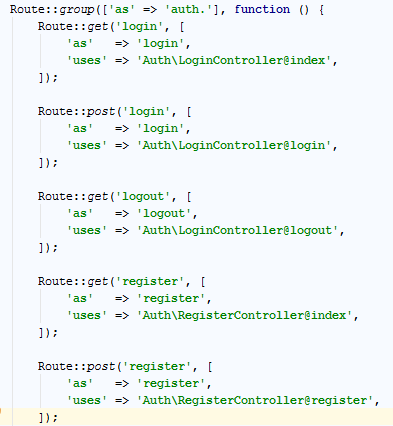
\includegraphics[width=\textwidth]{Images/Implementation/LaravelRouting}
    \caption{A subset of the routes defined in the authentication} \label{fig:Routes}
\end{figure}

Figure \ref{fig:Routes} shows the code which defines all the routes regarding the different user authentication components. The routes are grouped together with a prefix using the \emph{'as'} parameter. This adds the `\emph{auth::}' prefix to the name of each route. For example, using \emph{route(`auth::login')} will generate the URL pointing to the log-in page for user authentication. In addition to this, parameters can be included with a route request, allowing for more flexible URLs. Included parameters are passed to the relevant controller for the route. 

Routing with Laravel allows requests to be restricted to a certain type. With this, we can achieve security by limiting the type of HTTP request a route will accept. Laravel provides get, post, put, patch, and delete options for each route. A route defined using \emph{route::post} may only be accessed if the user posts form data to the URL. It is possible to bind a route to multiple request types such as get and post or even all request types but this is generally not recommended.

\subsection{Middleware}
HTTP middleware provides a convenient mechanism for filtering HTTP requests entering your application \cite{Laravel:Middleware}. Middleware is generally executed before a page is loaded in order to assess whether the user can access the page. It is possible to associate a page with multiple pieces of middleware, and this can be thought of as a chain of middleware - requirements being passed from a previous middleware triggers a call to the next one. A middleware can be assigned to a route, method, controller or even a group of middleware.

It is possible to create custom middleware using the Artisan utility. The \textit{php artisan make:middleware Demo} command will generate a middleware called Demo. The image in figure \ref{fig:MiddlewareTemplate} shows the template that is generated by the Artisan utility. The commented block on line 17 can be replaced with a check, which if passed allows the next middleware to be activated but if failed returns an alternative action to be executed. Middleware was used in Fidelis to achieve several trivial tasks in the application, each of which is discussed in the relevant sections through the rest of this chapter.

\begin{figure}[H]
    \centering
    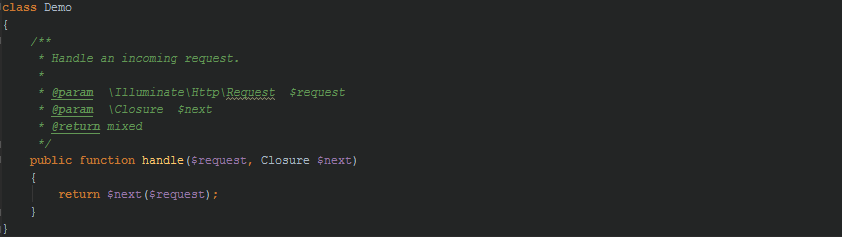
\includegraphics[width=\textwidth]{Images/Implementation/MiddlewareTemplate}
    \caption{Middleware Template Generated by the Artisan Utility} \label{fig:MiddlewareTemplate}
\end{figure}